\begin{savequote}[6cm]
<< The shape's fine, just make the whole thing... you know, cooler. 

\quad It needs to be about 20\% cooler. >>
\qauthor{Rainbow Dash}
\end{savequote}
\chapter{Gestion des préférences utilisateurs}\label{chap:prefs}
\chaptertoc

Grâce à la popularisation des technologies et des capacités de traitement de données, les systèmes sont de plus en plus complexes et fournissent de plus en plus de données. Le spectre des utilisateurs étant plus large, il est important de pouvoir adapter la masse d'informations récoltée à chaque personne. De nombreux efforts ont été consacrés ces dernières années à la personnalisation des réponses lors de l'accès aux bases de données. Dans ce chapitre, nous explorons une extension à notre approche pour ajouter des opérateurs adaptant les résultats d'interrogations aux préférences utilisateurs. Ainsi, l'utilisateur n'obtient que les données qui l'intéressent.

Dans la section~\ref{sec:ext:prefs:algebre}, nous détaillons les fondements théoriques à la gestion de préférences contextuelles. Une fois les opérateurs décrits dans l'algèbre Astral, nous pouvons présenter les algorithmes utilisés pour les mettre en œuvre dans la section~\ref{sec:ext:prefs:algo}. Enfin, dans la section~\ref{sec:ext:prefs:integration} nous présentons l'intégration faite dans Astronef pour que l'utilisateur puisse personnaliser ses résultats d'interrogation. Cette intégration est accompagnée d'une évaluation de performances pour sélectionner le meilleur algorithme de calcul.

\section{Modélisation algébrique}\label{sec:ext:prefs:algebre}
Dans cette section, nous introduisons dans le cadre d'Astral-Astronef les opérateurs de \textit{CPref-SQL}~\cite{DeAmo:cprefsql}. Tout d'abord, nous présentons les notions théoriques nécessaires pour appréhender les préférences contextuelles. Puis, nous présentons les deux opérateurs permettant de sélectionner les n-uplets préférés sur une relation temporelle. Ensuite, nous appliquons ceci à notre cadre applicatif. Enfin, nous présentons, comment l'intégration dans Astronef est faite.

\subsection{Préférences contextuelles}
Dans cette section nous présentons les principaux concepts concernant le formalisme logique que nous employons pour spécifier et raisonner avec des préférences. Tout d'abord, présentons le concept de préférence contextuelle. Une \textit{préférence contextuelle} est une manière d'exprimer la phrase suivante : \enquote{\it Lorsque $u$ est vrai, je préfère $Q_1$ à $Q_2$ à attributs $W$ égaux}. La définition~\ref{def:pref} définit formellement cette notion.

\begin{defi}[Préférence Contextuelle]\label{def:pref}
Soit $A$ un ensemble d'attribut,

Une \textit{règle de préférence contextuelle} (ou \textit{cp-règle}) sur $A$ est une formule $\varphi$ de la forme :
 $$\varphi: u \rightarrow Q_1(X) \succ Q_2(X)\ [W]$$
\begin{itemize}
	\item $X$ est un attribut non temporel de $R$ tel que $W \subseteq A$, $X \not \in W$,
	\item $Q_i(X)$ est une condition exprimée sur $X$,
	\item $\forall x$, $Q_1(x)$ et $Q_2(x)$ ne peuvent être satisfaites simultanément,
	\item $u$ est une condition ne portant ni sur $X$ ni sur les attributs de $W$.
	\end{itemize}
\end{defi}

La formule $u$ du côté gauche d'une cp-règle $\varphi$ est appelée \textit{contexte}. L'expression $Q_1(X) \succ Q_2(X)$ du côté droit est appelée \textit{expression de préférence} et les attributs dans $W$ sont appelés des attributs \textit{ceteris paribus} (cf. ci-dessous). Un n-uplet $s$ est dit \textit{compatible} avec une cp-règle $\varphi$ si $s$ satisfait son contexte.

Une \textit{théorie de préférence contextuelle} (\textit{cp-théorie}) sur $A$ est un ensemble fini $\Gamma$ de cp-règles sur $R$. Nous notons par Attr($\Gamma$) l'ensemble d'attributs dans les cp-règles de $\Gamma$.

Ainsi, une cp-règle $\varphi$ sur $A$ induit une \textit{relation binaire} (notée $\succ_\varphi$) sur une séquence de n-uplet d'attributs $A$, à savoir l'ensemble des paires ($s_1,s_2$) telles que $s_1$ est préféré à $s_2$ par rapport à $\varphi$. Cette relation binaire n'est pas nécessairement transitive, ce qui fait que ce n'est pas une \textit{relation d'ordre}. Nous définissons la notion de \textit{Relation de Préférence} inférée par une cp-théorie $\Gamma$.

\begin{defi}[Relation de Préférence]
Soit $\Gamma$ cp-théorie sur $A$,

La \textit{Relation de Préférence} associée à $\Gamma$ (notée $\succ_\Gamma$) est définie comme :
\begin{center} $\succ_\Gamma = (\cup_{\varphi \in \Gamma} \succ_\varphi)^*,$ o\`u $*$ dénote la \textit{fermeture transitive}.\end{center}
\end{defi}

Cette relation de préférence est dite \textit{consistante} si et seulement si elle est irréflexive. Si tel est le cas, elle devient ainsi une relation d'ordre partielle stricte. Des travaux existent pour vérifier si une cp-théorie est consistante~\cite{Wilson:cpnet}. Nous supposons pour la suite du document que nos relations le sont.

\subsection{Opérateurs de Préférences}
Les opérateurs de préférences calculent les données préférées par rapport à une cp-th\'eorie de référence. Chaque utilisateur donne au système ses préférences sous forme d'une cp-th\'eorie $\Gamma$ qui constitue ainsi une sorte de \textit{profil utilisateur} qui est évolutif. Concrètement, cette solution va permettre le support de requêtes 
\enquote{les plus préférées} et \enquote{les top-k} par l'intégration de deux opérateurs: \textbf{Best} et \textbf{KBest}.

L'opérateur \textbf{Best} sélectionne, dans relation temporelle ou non temporelle, les n-uplets qui correspondent le mieux à l'ensemble des préférences représentées dans $\Gamma$. D'un point de vue mathématique, il s'agit des n-uplets qui ne sont pas dominés dans la hiérarchie des préférences.

\begin{defi}[Best]\label{def:best}
Soit $R$ une relation temporelle et $\Gamma$ une cp-th\'eorie sur le schéma de $R$. 

\textbf{Best}$(R): b\mapsto \{u \in R(b) \mid \not\exists v \in r(t) \textrm{ tel que } v \succ_\Gamma u \}$
\end{defi}

L'opérateur \textbf{KBest} sélectionne les $k$ n-uplets qui correspondent au mieux à la hiérarchie des préférences énoncées dans $\Gamma$. Intuitivement \textbf{KBest}$_k(R)(b)$ retourne l'ensemble des $k$ n-uplets de $R(b)$ qui sont le moins dominés par d'autres n-uplets selon la hiérarchie de préférence. Pour définir sa sémantique, nous introduisons la notion de \textit{niveau} d'un n-uplet (noté $l(u)$) par rapport à une cp-théorie $\Gamma$ dans la définition~\ref{def:niveau}. Le niveau reflète l'écart entre ce n-uplet et ceux qui répondent complètement aux préférences de l'utilisateur.

\begin{defi}[Niveau]\label{def:niveau}
Soit $R$ une relation temporelle et $\Gamma$ une cp-th\'eorie sur le schéma de $R$.

Le \textit{niveau} de $u$, $l(u)$, \textit{par rapport à} $\Gamma$ au \textit{batch} $b$ est défini de manière inductive comme suit:
 \begin{itemize}
 \item Si $\not\exists u' \in R(b)$ tel que $u' \succ_\Gamma$ $u$, alors $l(u) = 0$.
 \item sinon $l(u)$ = $1+max \{l(u') \mid u' \succ_\Gamma u\} $
 \end{itemize}
\end{defi}

Il est possible de montrer que si $u \succ u'$ alors $l(u) < l(u')$. La réciproque n'est pas vraie. La sémantique de l'opérateur \textbf{KBest}$_k$ est présentée dans la définition~\ref{def:kbest}.

\begin{defi}[KBest]\label{def:kbest}
Soit $R$ une relation temporelle et $\Gamma$ une cp-th\'eorie sur le schéma de $R$. 

Pour un batch donné $b$, \textbf{KBest}$_k(R)(b)$ est l'ensemble des $k$ n-uplets $\in R(b)$ ayant le plus petit niveau. L'ordre positionnel est utilisé pour départager des n-uplets de même niveau.
\end{defi}

\subsection{Exemple de requête}
Supposons l'existence d'un flux $V$ agrégeant l'ensemble des informations \textit{volatiles}. Son schéma est le suivant : $V$(id, concept, type, volatile, value, $\t$). La description de ce schéma est l'expression suivante : l'entité de nature \textit{concept}, d'identifiant \textit{id} et de catégorie \textit{type} a émis la donnée de type \textit{volatile} et de valeur \textit{value} au temps $\t$. La formation de ce flux est triviale selon les principes développés en section~\ref{sec:valid:domvision:requetes} et n'est pas détaillé.

Nous souhaitons utiliser ce flux en tant que flux d'information à afficher à l'utilisateur. Afin de rapidement analyser l'activité du réseau, il souhaite obtenir une sélection des meilleures informations le concernant.

Soit $\Gamma$ la cp-théorie comportant les préférences contextuelles suivantes :
\begin{itemize}
	\item $\varphi_1 : $ volatile = cpu $\mapsto ($value $ \geq 90) \succ ($value $ < 90)$ [id]
	\item $\varphi_2 : $ $($volatile = status$) \succ ($volatile = cpu $ \vee $ volatile = mem$)$ [type]
	\item $\varphi_3 : $ concept = interface $\mapsto ($type = wifi$) \succ ($type = ethernet$)$
\end{itemize}

La figure~\ref{fig:valid:domvision:architecture:pref} représente un ensemble de données pour $V$. Si nous appliquons la relation d'ordre sur cet ensemble de n-uplet, nous pouvons remarquer que par la règle $\varphi_1$, nous obtenons que $s_1 > s_4$. Par $\varphi_2$ nous obtenons que $s_2 > s_1$. Et enfin, nous avons $s_3 > s_5$ par $\varphi_3$. La relation d'ordre $\succ_\Gamma$ est transitive, ainsi $s_2 > s_4$. Le graphe de la figure représente ces relations d'ordres.
\begin{figure}[ht]\centering
\begin{tabular}{|c|c|c|c|c|c|c|} \bottomrule
\rowcolor{hypcolor} $V$ & id & concept & type & volatile & value & $\t$\\ \hline
$s_1$ & 1 & equipement & gateway & cpu & 95 & 1\\ \hline % 1 > 4
$s_2$ & 2 & equipement & stb & status & 1 & 2\\ \hline % 2 > 1 > 4
$s_3$ & 3 & interface & wifi & bws & 150 & 3\\ \hline %
$s_4$ & 1 & equipement & gateway & cpu & 20 & 4\\ \hline
$s_5$ & 5 & interface & ethernet & bwr & 1200 & 5\\ \toprule % 3 > 5
\end{tabular}\hspace{1cm}
\begin{minipage}{3cm}
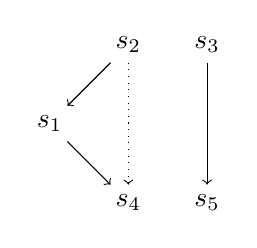
\begin{tikzpicture}[<-]
\node (sb) at (1,2) {$s_2$};
\node (sa) at (0,1) {$s_1$} edge (sb);
\node (sd) at (1,0) {$s_4$} edge (sa);

\draw (sd) edge [dotted] (sb);

\node (sc) at (2,2) {$s_3$};
\node (se) at (2,0) {$s_5$} edge (sc);
\end{tikzpicture}
\end{minipage}
\caption{Un jeu de données pour $V$ et son graphe de préférence correspondant}\label{fig:valid:domvision:architecture:pref}
\end{figure}

En supposant que nous appliquons une fenêtre sur $V$ et que nous obtenons les n-uplets présentés au batch $b$. Nous obtenons les résultats suivants : 
\begin{itemize}
	\item \textbf{Best}$(R)(b) = \{s_2,s_3\}$, car ces deux n-uplets ne sont pas dominés.
	\item \textbf{KBest}$_3(R)(b) = \{s_1,s_2,s_3\}$ par sélection du niveau 0 et 1.
	\item \textbf{KBest}$_4(R)(b) = \{s_1,s_2,s_3,s_4\}$, car $s_5$ est arrivé après $s_4$ et l'ordre positionnel domine à niveau équivalent.
\end{itemize}

Dans la pratique nous pourrions appliquer cet opérateur sur tout type de fenêtre. Pour revenir à notre application, en supposant que $V$ est correctement formé, nous pouvons déployer une requête continue qui peut alimenter l'interface de l'utilisateur avec : les 25 événements les plus importants du dernier jour évaluée toutes les minutes. Cette requête a l'expression $\textbf{KBest}_{25}(V[T\ 1j\ 1min])$.

Nous avons désormais présenté les deux opérateurs nous permettant la personnalisation de résultat. Dans la section suivante, nous détaillons leur implémentation.

\section{Mise en œuvre}\label{sec:ext:prefs:algo}
Cette section présente les algorithmes que nous avons développés pour les opérateurs \textbf{Best} et \textbf{KBest}. Ces opérateurs nécessitent de connaître la hiérarchie des n-uplets déduite d'un ensemble de préférences. Cette hiérarchie est déduite du \textit{graphe de préférence} \textit{GP}. Nous présentons ci-après deux algorithmes pour la gestion du graphe : l'un est calculé sur l'état courant de la relation temporelle d'entrée, l'autre travaille sur les différences de la relation temporelle de manière incrémentale.

\subsection{Le graphe de préférence}
L'ordre de préférence entre deux n-uplets $t_1$ et $t_2$ selon une règle $\varphi$ est construit à partir d'une fonction $Com\-pare(t_1,t_2,\varphi_k)$ qui retourne $\emptyset$ si $t_1$ et $t_2$ sont incomparables, 1 si $t_1$ est préféré à $t_2$ et $-1$ sinon. L'algorithme~\ref{algo:comparT} étend la comparaison à une théorie $\Gamma$. Cette dernière utilise un ensemble de règles pour calculer l'ordre de préférence, mais ne calcule pas la clôture transitive.

\textbf{Graphe de préférence : }
Les opérateurs \textbf{Best} et \textbf{KBest} sont appliqués sur un ensemble de n-uplets $TS$ et ont besoin du graphe de préférence relatif à $TS$.
Pour son implémentation, nous avons adopté la structure $Graph(Next, Prec, Src)$ défini comme suit:
 $Next$ associe chaque n-uplet à la liste des n-uplets \textbf{qu'il domine}.
 $Prec$ associe chaque n-uplet à la liste des n-uplets \textbf{qui le dominent}.
 $Src$ est l'ensemble des n-uplets non dominés, représentant la source du graphe.
Afin de fournir de bonnes performances, les implémentations de ces structures sont des \textit{hash-sets} ou \textit{hash-maps}.

La construction et la mise à jour du graphe utilisent des méthodes \textit{Graph.Insert} et \textit{Graph.Delete} qui fonctionnent comme suit. Pour insérer un n-uplet dans un graphe, la méthode \textit{Graph.Insert} itère sur les nœuds du graphe pour mettre à jour \textit{Next}, \textit{Prec} et l'ensemble \textit{Src}. Comme le coût de l'insertion et de suppression dans une structure hachée peut être considéré comme $\mathcal O(1)$, le coût global de l'insertion d'un n-uplet dans le graphe est de $\mathcal O(\abs G)$. Pour la suppression d'un n-uplet $s$ du graphe, la méthode \textit{Graph.Delete} itère sur les n?uds connectés à $s$. Le coût est de $\mathcal O(\mathrm{deg}(s))$.

Pour une théorie de préférences $\Gamma$ donnée et un ensemble de n-uplets $TS$, la construction du graphe de préférence complet est réalisée par l'algorithme~\ref{algo:create}.

\subsection{Calcul de Best et KBest}
Par définition, le graphe inclut l'ensemble $Src$ qui contient les n-uplets les plus préférés. L'ensemble $Src$ est le résultat de l'opérateur \textit{Best}. Toutefois, l'algorithme peut-être optimisé en évitant de construire complètement \textit{GP}. La méthode $Graphe.Insert$ peut être optimisée pour tenir compte de cela. 
La complexité est alors réduite à $\mathcal O(\abs{Src})$. La complexité de $Best(R)(b)$ devient $\mathcal O(NS)$ où $N = \abs{R(b)}$ et $S=\abs{Best(R)(t)}$.

L'algorithme principal utilisé pour calculer $KBest$ à partir du \textit{GP} est un tri topologique de Kahn limité aux $k$ premiers résultats. Voir l'algorithme~\ref{alg:kbest}.

\subsection{Évaluation incrémentale du GP}
Cette section présente un algorithme pour le calcul incrémental de \textit{GP}. Le fait que les requêtes avec préférences sur les flux s'expriment sur des séquences de fenêtres motive cette méthode. Il est nécessaire de construire le \textit{GP} pour l'ensemble des n-uplets de la fenêtre \textit{courante}. Comme deux fenêtres consécutives peuvent se superposer, le nouveau \textit{GP} peut être construit par mise à jour incrémentale du graphe \textit{courant}. 

Supposons que $\delta_R^{-}$ contienne les n-uplets \textit{sortants} de la fenêtre et $\delta_R^{+}$ contienne ceux qui \textit{rentrent} dans la nouvelle fenêtre. Il n'y a pas d'intersection entre ces deux ensembles. Ces ensembles sont utilisés par l'algorithme~\ref{algo:update} pour construire le \textit{GP} de la nouvelle fenêtre à partir du \textit{GP} de la précédente. 

Il est important de noter que l'approche incrémentale est intéressante si la différence entre deux graphes successifs est faible comparée à la taille totale du graphe. Dans un tel cas, une grande proportion du \textit{GP} est réutilisée. Dans le cas contraire, la création du \textit{GP} \textit{de zéro} est meilleure. Le tableau~\ref{tab:valid:perfs:prefs:complexity} résume l'ensemble des complexités algorithmiques.

\begin{table}[p]
\noindent
\begin{minipage}{0.55\textwidth}
\small
\begin{algorithm}[H]\caption{Calcule KBest$(R)(t)$}\label{alg:kbest}
\dontprintsemicolon
\KwData{La structure GP, $k$ le nombre de n-uplet demandé}
Res $\gets $ \textbf{new TreeSet}$()$ \tcp{Ensemble ordonné}
\If{$k < \abs{Src}$}{\tcp{Src contient plus de $k$ n-uplets}
	$N \gets \abs{Src} - k$ \;\tcp{L'ordre position de Src est utilisé}
	\ForEach{$s\in Src$}{\tcp{ pour garder les $k$ n-uplets les plus récents}
		\lIf{$N = 0$}{Res.add$(s)$\;}
		\lElse{$N \gets N-1$\;}
	}
	\Return{Res}
}
NextLvl $\gets Src$; $id \gets 0$\;
PrecCount $\gets $ \textbf{new HashMap}()\;
\While{$id<k$ \textbf{and} $id < \abs{Src}+$Prec.count()}{
	\tcp{Buffer contient les n-uplets du même niveau}
	\If{Buffer = $\emptyset$}{
		\ForEach{$t\in $NextLvl}{
			Buffer.push$(t)$\;
		}
		NextLvl.clear()\;
	}
	$t\gets$ Buffer.pop()\;
	\ForEach{$s\in Next$.get$(t)$}{\tcp{Pour tout n-uplet dominé par $t$}
		$n\gets $PrecCount.get$(s)$\;
		\If{$n = $\textbf{null}}{$n=$Prec.get$(s)$.size()\;}
		\If{$n=1$}{
			NextLvl.add$(s)$\;\tcp{$s$ fait parti du prochain niveau}
		} \lElse {
			PrecCount.put$(s,n-1)$\;\tcp{Il n'y a plus de nœud dans cet ensemble}
		}
	}
	Res.add$(t)$\;
}
\Return{Res}
\end{algorithm}
\end{minipage}
\begin{minipage}{0.45\textwidth}
\small

\begin{algorithm}[H]\caption{ComparT$(t_1,t_2,\Gamma)$}\label{algo:comparT}
\dontprintsemicolon
%\begin{algorithmic}
%\KwIn{$t_1$ and $t_2$ two tuples from $R$}
\KwData{$\Gamma = \{\varphi_1,...,\varphi_k\}$ une théorie}
\KwResult{$\{1,-1,\emptyset\}$, \\ \quad resp. $\{t_1 >_{\Gamma} t_2$, $t_1 <_{\Gamma} t_2$, inc.$\}$}
\ForEach {$\varphi_k \in \Gamma$}{
	$r\gets Compare(t_1,t_2,\varphi_k)$\;
\lIf{$r \neq \emptyset$}{
\Return{$r$}
}
}
\Return{$\emptyset$}
%\end{algorithmic}
\end{algorithm}

\vspace{1cm}
\begin{algorithm}[H]\caption{Créer GP}\label{algo:create}
\dontprintsemicolon
\KwIn{$TS$ un ensemble de n-uplets}
\KwData{La structure de GP}
\lForEach{$s\in TS$}{
	$Graph.$insert$(s)$\;
}
\end{algorithm}

\vspace{1cm}
\begin{algorithm}[H]\caption{GP incrémental}\label{algo:update}
\dontprintsemicolon
\KwIn{$\delta_R^{-}(t,i)$ and $\delta_R^{+}(t,i)$}
\KwData{La structure du GP}
\lForEach{$s\in \delta_R^{-}(t,i)$}{
	$Graph.$Delete$(s)$\;
}
\lForEach{$s\in \delta_R^{+}(t,i)$}{
	$Graph.$Insert$(s)$\;
}
\end{algorithm}

\vspace{1cm}
\begin{tabular}{rcc}
& Créer GP & GP Incrémental\\ \noalign{\hrule height 1pt}
Best \quad &\quad $\mathcal O(N.S)$\quad & $\mathcal O(\Delta.N)$ \\
KBest \quad & $\mathcal O(N^2)$ & \quad $\mathcal O((\Delta+k)N)$ \quad\\ \noalign{\hrule height 1pt}
\end{tabular}
\caption{Complexité de Best/KBest}\label{tab:valid:perfs:prefs:complexity}
\end{minipage}
\end{table}

\section{Intégration de nouveaux composants}\label{sec:contrib:astronef:integration}
Astronef est basé sur l'architecture de composants orientés services. Ainsi, nous pouvons apporter de nouveaux composants à l'exécution. Toutefois, l'intégration des composants opérateurs nécessite aussi l'apport de ses connaissances en terme de règles logiques. L'intergiciel expose un service \textit{KnowledgeBase} capable d'ajouter des règles à sa base de connaissance (sous forme de fichier ou de chaînes de caractères). Ainsi, le constructeur de requête est lui aussi extensible.

Afin d'être compatible le composant doit fournir la fabrique dans la même technologie que les opérateurs originels (en l'occurence iPojo/OSGi). Il doit naturellement aussi fournir les services nécessaire à son exploitation. Enfin, il doit spécifier les propriétés de configurations qu'il supporte, et évidemment respecter et correctement manipuler les services d'Astronef pour manipuler les structures de données ou le \textit{Scheduler}.

La seule règle obligatoire pour exploiter un nouveau composant est de fournir au moins une règle \textbf{implrules} où le nom du composant (sa classe d'implémentation par défaut) est indiqué. Si ce composant implémente un macro-bloc, alors il faut définir potentiellement un nouveau nom de nœud en plus des règles \textbf{macrobloc}.

Mais si ce composant implémente un nouvel opérateur que nous souhaitons utiliser dans l'expression de requête. Alors il est strictement \textbf{nécessaire} de définir sa sémantique en terme de types supportés et d'attributs fournis. Sans ces deux règles, il est impossible de construire la requête. De plus, si nous possédons la connaissance suffisante, nous pouvons indiquer son comportement face à la projection, la sélection ou d'autres optimisations logiques.

\section{Conclusion}
Ce chapitre a dressé un état de l'art des différents systèmes capables d'offrir une solution générique de supervision. Il en ressort qu'aucun système ne supporte entièrement les critères de qualité que nous nous sommes fixés. Le tableau~\ref{tab:rw:supervision:bilan} résume les 11 points d'analyse en colorant les différentes points suivant leurs conformités. 

\begin{sidewaystable}[ht]
\centering
\begin{tabular}{@{{\vrule width 1pt}\ \ }>{\raggedleft}m{3cm}@{\ \ {\vrule width 1pt}\ \ }M{4.2cm}|M{4.2cm}|M{4.2cm}|M{4.2cm}@{\ \ {\vrule width 1pt}}} \bottomrule
\head Critère & \head Système d'administration & \head Gestion de contexte & \head Entrepôts de données & \head Gestion de flux de données \\  \toprule \bottomrule
\critereAA & Hiérarchique & Triplets & Relationnel & Relationnel dérivé \\ \hline
\critereAB & \meh Structure hiérarchique sans contraintes & \good Ontologies & \good Modèle relationnel normalisé & \bad Pas de structure \\ \hline
\critereAC & \meh Notifications & \bad Ajout du temps en propriété & \meh CDC & \good Flux natif \\ \toprule \bottomrule
\critereBA & \meh Instantanée, continu en ad-hoc & \bad Instantané principalement & \meh Instantané. ETL en pseudo-continu & \bad Continu uniquement \\ \hline
\critereBB & \good Standardisation, union de modèles & \meh Fusion d'ontologies non standardes & \good Processus ETL (complexe) & \good Union et jointures de flux \\ \hline
\critereBC & \bad Impératif principalement & \good Logique & \meh Déclaratif (SQL) et Procédural (ETL) & \good Déclaratif principalement\\ \hline
\critereBD & \meh Procédures à écrire soi-même & \good Logique du premier ordre & \good Relationnel multidimensionnel et Algorithmie dédiée & \meh Relationnel avec support du dynamisme\\ \toprule \bottomrule
\critereCA & \good Support des standards & \meh Spécification longue des domaines & \bad Spécification du schéma, des ETL, autre (complexe) & \good Écriture de requêtes \\ \hline
\critereCB & \bad Aucune & \good Séparation par les domaines & \good Données multidimensionnelles & \bad Aucune \\ \hline
\critereCC & \good Modèle extensible, fonctions métiers dans le gestionnaire & \meh Capteurs virtuels & \good Opérateurs ETL, procédures SQL, algorithmes & \meh Sources et puits mais pas les opérateurs  \\ \hline
\critereCD & \good Large échelle & \bad Complexité très haute & \meh Réactivité lente, Support de grande quantité & \good Support de haut débits\\ \toprule 
\end{tabular}
\caption{Récapitulatif de l'état de l'art des systèmes génériques de supervision}\label{tab:rw:supervision:bilan}
\end{sidewaystable}
Il en ressort que les systèmes d'administrations sont avant tout des systèmes qui fonctionnent grâce au support des standards et à leur simplicité d'implémentation. L'architecture avec gestionnaire adaptable grâce à des langages impératifs permets une grande flexibilité pour s'adapter aux cas d'usages. De son côté, l'informatique contextuelle fournit des outils permettant de modéliser et manipuler proprement les concepts du système grâce aux ontologies et aux raisonnements logiques. Il en sort une claire séparation des domaines de compétences. Les entrepôts de données quant à eux se distinguent par des capacités d'analyses très poussées, ainsi qu'un procédé d'intégration, très complexe et lourd malheureusement, mais très complet. Enfin, la gestion de flux de données est une base solide pour gérer les données dynamiques. L'intégration et l'adaptation au système étant fait entièrement de manière déclarative en fait une solution performante et viable.

À la vue de l'état de l'art, voici les points qui vont être critique sur notre établissement de notre contribution :
\begin{itemize}
    \item La gestion de flux est un bon socle pour gérer les données dynamique grâce aux requêtes continues.
    \item Elle ne suffit pas pour constituer un système d'observation complet, notamment à l'absence de modèle de description et de requêtes instantanées.
    \item Les entrepôts et bases de données sont capables de répondre aux requêtes instantanées.
    \item Les ETL sont trop complexes à manipuler pour intégrer les données, alors que les SGFD sont plus déclaratifs.
\end{itemize}
Il devient clair que les systèmes de gestions de flux de données forment un bon candidat comme fondation pour un architecture d'observation de système. Il nous faut donc approfondir l'état de l'art technique sur ce domaine pour modeler notre contribution. Le point majeur sera d'apporter les capacités des systèmes de gestions de données relationnels. En effet, en apportant le support persistant à la gestion de flux de données, en clarifiant et augmentant son langage, nous aurons un outil qui sera plus apte à répondre à notre problématique. Ainsi, l'héritage du relationnel permettra une structure sémantique correcte, ainsi que des capacités d'analyses plus évoluées. Enfin et surtout, les données serait intégrés malgré leur hétérogénéité profonde. Le chapitre suivant détaille l'état de l'art technique de la gestion de flux de données afin de pouvoir effectuer ces améliorations.
